\documentclass[12pt]{article}
\usepackage{times}
\usepackage{graphicx}
\usepackage{lineno}
\usepackage{multirow}
\usepackage[english]{babel}
\usepackage{hyperref}
\usepackage{typearea} 
\usepackage{amssymb}
\usepackage{amsfonts}
\usepackage{amsmath}
\usepackage{color}

\renewcommand{\baselinestretch}{1.2}
\newcommand{\bbar}[1]{\overline{#1}}

\title{\vspace*{-22mm}\bf Electronic supplementary material: Mutualism and evolutionary multiplayer games}
\author{Chaitanya S.~Gokhale$^{\ast}$ and Arne Traulsen\\
\vspace{-2mm}\normalsize  Research Group for Evolutionary Theory,\\
\vspace{-2mm}\normalsize  Max-Planck-Institute for Evolutionary Biology\\
\vspace{-2mm}\normalsize  August-Thienemann-Stra{\ss}e 2, 24306 Pl\"{o}n, Germany\\
\vspace{-2mm}\normalsize $\ast$ Corresponding author, gokhale@evolbio.mpg.de} 
\date{\normalsize\today}

\begin{document}

\linenumbers
\maketitle


\section*{
Evolutionary games within a species and between two species
}
\subsection*{Evolutionary games within a single species}
\label{withinsp}
In evolutionary game theory two player games with two strategies have been studied in great detail in infinitely large populations.
Typically, two players meet, interact and obtain a payoff. 
The payoff is then the basis for their reproductive success and hence for the change in the composition of the population \cite{maynard-smith:book:1982}.
Consider two strategies, $G$ and $S$.
We define the payoffs by $a_{i,j}$ where $i$ is the strategy of the focal individual and $j$ is the strategy of the other interacting individual.
For example, when an $G$ strategist meets another person playing $G$ she gets $a_{G,G}$.
She gets $a_{G,S}$ when she meets a $S$ strategist.
This leads to the payoff matrix
%
\begin{equation}\label{eq:twobytwo}
\begin{array}{ccc}
\hline\hline
 &$G$	&	$S$\\
\hline
$G$ 	& a_{G,G} &	a_{G,S} 
 \\
 $S$ 	&  a_{S,G} &a_{S,S} \nonumber \\
 \hline\hline
\end{array}
\end{equation}
%
The average payoffs for the two strategies are given by, %
\begin{eqnarray}
f_{G_1} (x) &= a_{G,G} x + a_{G,S} (1-x) \nonumber \\
f_{S_1} (x) &= a_{S,G} x + a_{S,S} (1-x), \nonumber
\end{eqnarray}
%
where $x$ is the frequency of the players with strategy $G$.
Typically these average payoffs are directly considered as the average fitnesses of the two strategies.
This framework is used for biological systems, where strategies spread by genetic reproduction and often also for social systems where strategies spread by imitation.
The concept is valid for interactions within a species where the evolutionary dynamics of strategies within the species is of interest.
But quite often, interactions are not between two players, but between whole groups of players. 
Quorum sensing,  group hunting or climate preservation represent such multiplayer examples.
Such multiplayer games have been analyzed in the context of the evolution of cooperation \cite{hardin:Science:1968,hauert:PRSB:1997,kollock:ARS:1998,rockenbach:Nature:2006,milinski:PNAS:2006,milinski:PNAS:2008}, but only recently in a  more general sense \cite{pacheco:PRSB:2009,kurokawa:PRSB:2009,souza:JTB:2009,gokhale:PNAS:2010}.
The complexity brought to the table by such multiplayer interactions can be illustrated by adding just one more player in the previous setup.
Now instead of a two player game if we have a three player game then the payoff table is,
%
\begin{equation}\label{eq:threepl}
\begin{array}{cccc}
\hline\hline
 &$GG$	&	$GS$		&	$SS$\\
\hline
$G$ 	& a_{G,G,G} &	a_{G,G,S} &	a_{G,S,S} 
 \\
 $S$ 	&  a_{S,G,G} &a_{S,G,S}  &a_{S,S,S} \nonumber \\
 \hline\hline
\end{array}
\end{equation}
%
The fitnesses of the two types in such a case are given by,
\begin{eqnarray}
f_{G_1} (x) &= a_{G,G,G} x^2 + 2 a_{G,G,S} x (1-x) + a_{G,S,S} (1-x)^2 \nonumber \\
f_{S_1} (x) &= a_{S,G,G} x^2 + 2 a_{S,G,S} x (1-x) + a_{S,S,S} (1-x)^2 \nonumber
\end{eqnarray}
where the nonlinearity of order two comes from the fact that each focal individual interacts with $2$ other individuals.
Since we assume that the order of players does not matter we get a binomial coefficient of $2$ when playing with two individuals with different strategies. 

\subsection*{Evolutionary games between two species}
The above section was the traditional way of analyzing evolutionary games (either two or multiplayer) within a species but when species interact then we need to formalize the interactions in a different manner.
Just as in the previous section the average fitnesses were a function of the frequency of the strategies within the species ($f(x)$), here we assume that fitness depends on the frequency of the strategies in the other species ($f(y)$).
It is indeed possible to incorporate even more complexity by making the fitness depend on both the frequencies of strategies within the species and from the other species but that case is much more complicated and beyond the scope of this paper. 
Interested readers are referred to \cite{schuster:BC:1981c}.
For simplicity we stick to the assumption from coevolutionary models of interspecific dependence only \cite{roughgarden:TPB:1976,roughgarden:book:1983}.


For two player games between species (Fig. \ref{fig:concept} A)  now we need to pick one individual from each species and they play the game.
For simplicity we assume that both the populations have the same strategies $G_i$ and $S_i$ but now we use subscript to define the species they come from $i = (1,2)$. 
Thus the payoff matrices describing the interactions
are,
\begin{equation}\label{}
\begin{array}{cccc}
& & \multicolumn{2}{c}{\text{Species 2}}\\
\hline\hline
&	&	G_2		&	S_2	\\
\hline
 \multirow{2}{*}{Species 1} & G_1 	& a_{G_1,G_2} &	a_{G_1,S_2} \\
&	S_1	&  a_{S_1,G_2} & a_{S_1,S_2} \\
 \hline\hline
\end{array}
\hspace{1cm}
\begin{array}{cccc}
& & \multicolumn{2}{c}{\text{Species 1}}\\
\hline\hline
&	&	G_1		&	S_1	\\
\hline
 \multirow{2}{*}{Species 2} & G_2 	& a_{G_2,G_1} &	a_{G_2,S_1} \\
&	S_2	&  a_{S_2,G_1} & a_{S_2,S_1} \nonumber \\
 \hline\hline
\end{array}
\end{equation}
with the respective average fitnesses now being,
\begin{eqnarray}
f_{G_1} (y) &= a_{G_1,G_2} x + a_{G_1,S_2} (1-x) \hspace{1cm} f_{G_2} (x) = a_{G_2,G_1} x + a_{G_2,S_1} (1-x)\nonumber \\
f_{S_1} (y) &= a_{S_1,G_2} x + a_{S_1,S_2} (1-x) \hspace{1cm} f_{S_2} (x) = a_{S_2,G_1} x + a_{S_2,S_1} (1-x) .\nonumber
\end{eqnarray}
Increasing the number of players in now an additional complication. 
Hence, we proceed by an addition of one more player in just one of the species to illustrate the intricacy.
Let us assume that Species $1$ is playing a two player game while Species $2$ plays a three player game (see Fig. \ref{fig:concept} B).
This means that we need to pick one individual each from the two species to make up the two player game but we need two individuals from Species $1$ and $1$ from Species $2$ to make up the three player game.
This is because we have neglected intraspecific interactions as mentioned earlier.
If both the Species play a three player game (see Fig. \ref{fig:concept} C) then we pick two player from each species and the games are again without including intraspecific interactions.
\begin{equation}\label{}
\begin{array}{ccccc}
& & \multicolumn{3}{c}{\text{Species 2}}\\
\hline\hline
& & G_2 G_2	&	G_2 S_2		&	S_2 S_2\\
\hline
 \multirow{2}{*}{Species 1} & G_1 	& a_{G_1,G_2,G_2} &	a_{G_1,G_2,S_2} &	a_{G_1,S_2,S_2} 
 \\
 & S_1 	&  a_{S_1,G_2,G_2} &a_{S_1,G_2,S_2}  &a_{S_1,S_2,S_2} \\
 \hline\hline
\end{array}
\hspace{0.5cm}
\begin{array}{ccccc}
& & \multicolumn{3}{c}{\text{Species 1}}\\
\hline\hline
& & G_1 G_1	&	G_1 S_1		&	S_1 S_1\\
\hline
 \multirow{2}{*}{Species 2} & G_2	& a_{G_2,G_1,G_1} &	a_{G_2,G_1,S_1} &	a_{G_2,S_1,S_1} 
 \\
 & S_2 	&  a_{S_2,G_1,G_1} &a_{S_2,G_1,S_1}  &a_{S_2,S_1,S_1} \nonumber \\
 \hline\hline
\end{array}
\end{equation}
and the respective average fitnesses are,
\begin{eqnarray}
f_{G_1} (y) &= a_{G_1,G_2,G_2} y^2 + 2 a_{G_1,G_2,S_2} y (1-y) + a_{G_1,S_2,S_2} (1-y)^2  \nonumber \\
f_{S_1} (y) &= a_{S_1,G_2,G_2} y^2 + 2 a_{S_1,G_2,S_2} y (1-y) + a_{S_1,S_2,S_2} (1-y)^2 \nonumber \\
f_{G_2} (x) &= a_{G_2,G_1,G_1} x^2 + 2 a_{G_2,G_1,S_1} x (1-x) + a_{G_2,S_1,S_1} (1-x)^2 \nonumber \\ 
f_{S_2} (x) &= a_{S_2,G_1,G_1} x^2 + 2 a_{S_2,G_1,S_1} x (1-x) + a_{S_2,S_1,S_1} (1-x)^2.\nonumber
\end{eqnarray}

%For different types of interactions between species differrent models need to be defined \cite{poulin:JTB:1995,doebeli:PNAS:1998,noe:book:2001,johnstone:ECL:2002,bergstrom:PNAS:2003,hoeksema:AmNat:2003,akcay:PRSB:2007,bshary:Nature:2008}.
\begin{figure}
\begin{center}
%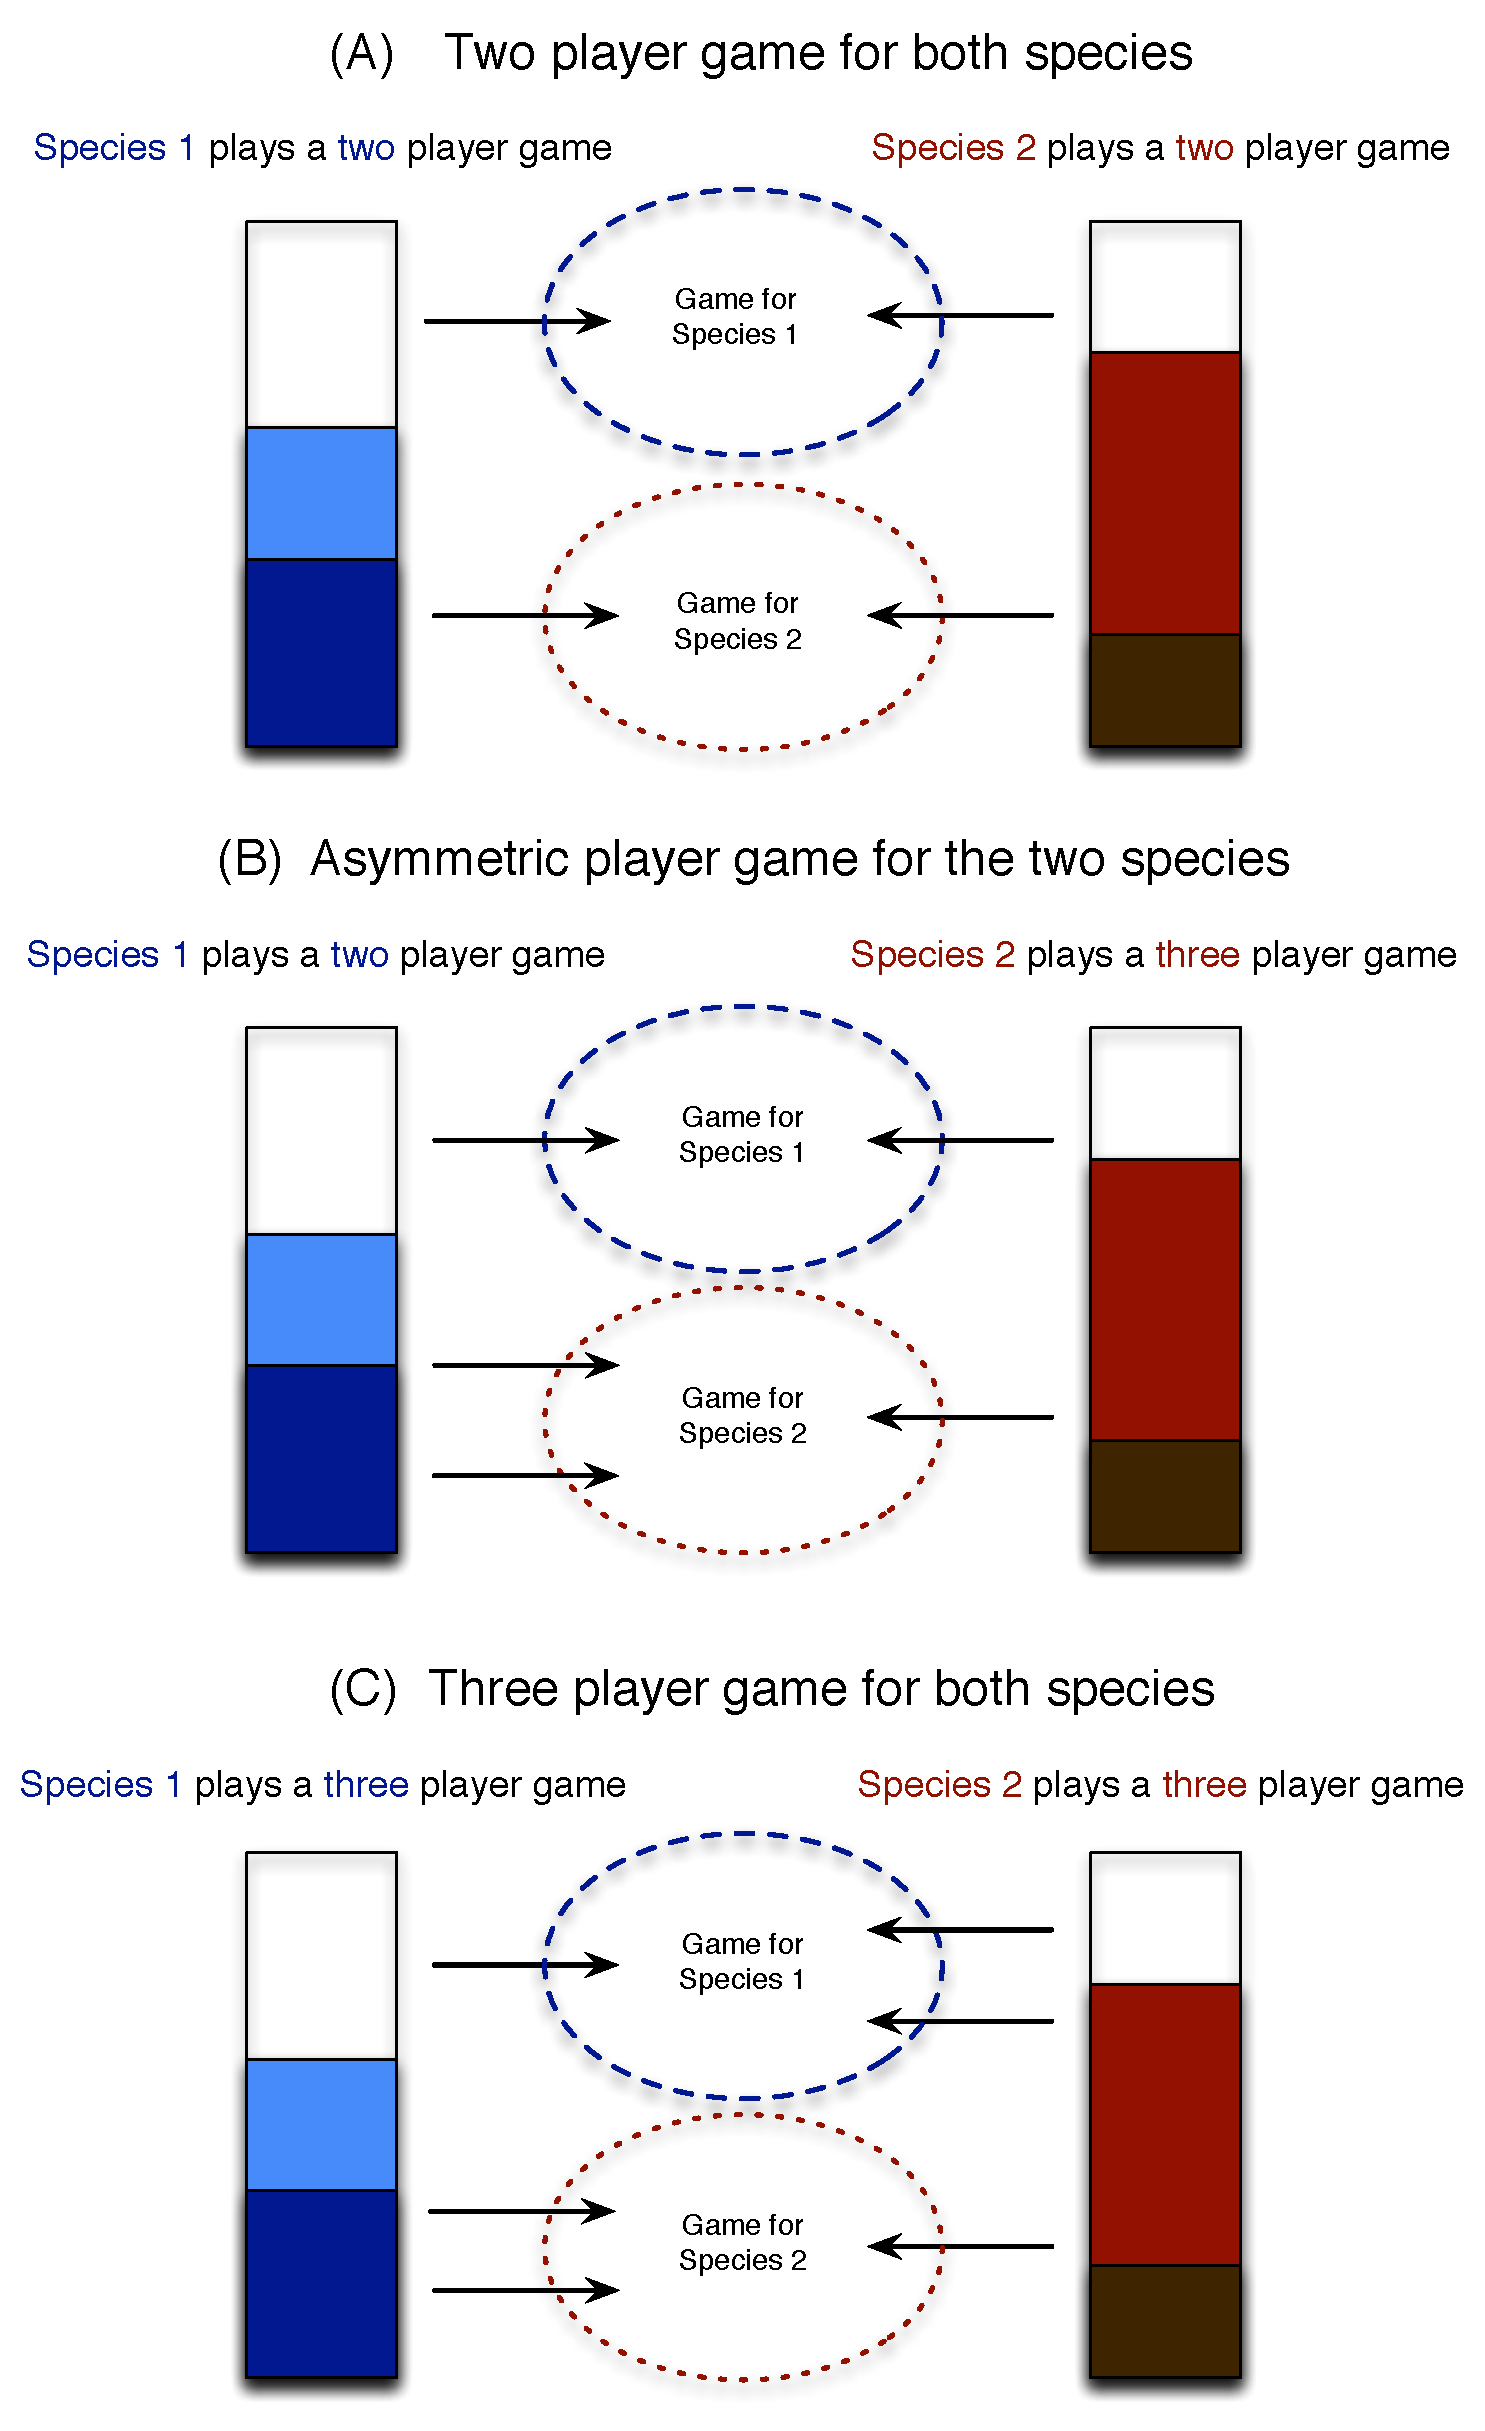
\includegraphics[scale=0.4]{concept.eps}
\end{center}
\caption{
Evolutionary games between two species.
(A) If both the species are playing a two player game then from either species we choose one player each to play the game.
(B) Species $1$ plays a two player game, hence the for this pairwise interaction we choose a single species two player to interact with a single species $1$ player (blue dashed oval). Species $2$ plays a three player game, hence one player of species $2$ interacts with two individuals of species $1$ (red dotted oval).
(C) If both species are playing a three player game then for a single individual of Species $1$ we pick two players from Species $2$ (blue dashed oval) and vice versa for a single individual of Species $2$ (red dotted oval).
}
\label{fig:concept}
\end{figure}




\section*{The snowdrift game}
\label{appA}
\subsection*{Two player setting}
So far, we have described general games within and between species, now we turn to a particular game which of interest to us when considering mutualism.
The snowdrift game derives its name from the anecdote where two drivers are stuck in a snowdrift.
They must shovel away the snow (paying the cost $c$) to reach home (benefit $b$) but there are three possible outcomes to this scenario.
One of the driver shovels while the other stays warm in the care ($b-c$ and $b$), both the drivers share the workload and shovel away the snow ($b-c/2$ and $b-c/2$) or none of them gets out of the care and they both remain stuck ($0$ and $0$).

Putting this game in perspective of the two species (i.e. the two drivers represent the two different species) we get the matrix,\\
%
\begin{equation}\label{}
\begin{array}{cccc}
& & \multicolumn{2}{c}{\text{Species 2}}\\
\hline\hline
&	&	G_2		&	S_2	\\
\hline
 \multirow{2}{*}{Species 1} & G_1 	& b-c/2 &	b-c \\
&	S_1	&  b & 0 \\
 \hline\hline
\end{array}
\hspace{1cm}
\begin{array}{cccc}
& & \multicolumn{2}{c}{\text{Species 1}}\\
\hline\hline
&	&	G_1		&	S_1	\\
\hline
 \multirow{2}{*}{Species 2} & G_2 	& b-c/2 &	b-c \\
&	S_2	& b & 0 \nonumber \\
 \hline\hline
\end{array}
\end{equation}
%
where strategy $G$ stands for being \textit{``Generous"} and shoveling the snow while $S$ stands for being \textit{``Selfish"} and just sitting in the car.
For $b=2$ and $c=1$ we recover the matrix used in \cite{bergstrom:PNAS:2003}.

For the snowdrift game in a single population there exists a single, stable internal equilibrium.
Hence the population will evolve to a polymorphism which is a combination of \textit{``Generous"} and \textit{``Selfish"} individuals.
But in a two species system, this stable equilibrium turns into a saddle point, a small deviation from this fixed point can lead the system to one of the stable fixed point where one of the species is completely \textit{``Generous"} 
and the other one is completely \textit{``Selfish"}.

\subsection*{Multiplayer setting}
\label{appB}

Following Souza et al. \cite{souza:JTB:2009},  
a multiplayer snowdrift game can be described by the payoff entries
\begin{align}
\Pi_{G_1} (k) & = \begin{cases} b-\frac{c}{k} & \textrm{if } k \geq M \\  -\frac{c}{M} & \textrm{if } k < M \end{cases}
\\
\Pi_{S_1} (k) & = \begin{cases} b & \textrm{if } k \geq M \\ 0 & \textrm{if } k < M. \end{cases}
\end{align}
%
The selfish players get the benefit $b$ if the number of generous individuals in both species combined, $k$, is greater than or equal to the threshold $M$.
For the generous individuals, their effort is subtracted from the payoffs.
The effort is shared if the quorum size is met ($\frac{c}{M}$), but is in vain for $k<M$.
For two player games we had $k=1$ but multiplayer games provide the possibility of exploring this threshold aspect of collective action games.
From these payoff entries we need to calculate the average fitnesses.
For simplicity we just illustrate the fitnesses of the strategies in Species $1$.
Just like in a three player game for Species $1$ we needed to pick two individuals from Species $2$, for a $d$ player game for Species $1$ we need to pick $d-1$ other individuals from Species $2$ (See Fig. \ref{fig:concept} C).
We assume that the groups are randomly assembled from the composition of Species $2$.
Indeed due to this random sampling the composition of the formed groups is given by a binomial distribution.
Summing over all possible compositions of groups we arrive at  the average fitnesses of the two strategies in species $1$,
%
\begin{align}
f_{G_1} (y) &= \sum_{k=0}^{d-1} \binom{d-1}{k}y^k (1-y)^{d-1-k} \Pi_{G_1}(k+1) \\
f_{S_1} (y) &= \sum_{k=0}^{d-1} \binom{d-1}{k}y^k (1-y)^{d-1-k} \Pi_{S_1}(k).
\label{fiteqs}
\end{align}
%
Following the same procedure for the two strategies in species $2$ leads to the average fitness of the two species
%
\begin{align}
\bar{f}_1 (x,y) &= x f_{G_1} (y)+(1-x) f_ {S_1}(y)\\
\bar{f}_2 (x,y) &= y f_{G_2} (x)+(1-y) f_{S_2}(x).
\label{avgfiteqs}
\end{align}
%

\section{Dynamics in asymmetric conditions}

We have addressed two kinds of asymmetries in the game, the number of player and the thresholds in the two species.
We denote the number of players for species $1$ and species $2$ as $d_1$ and $d_2$, respectively.
That is if species $2$ is playing a $d_2$ player game it means that one player from species $2$ interacts with $d_2-1$ players of species $1$ (for e.g.	Fig \ref{fig:concept} B).
For an asymmetry in the thresholds we use the two parameters $M_1\geq1$ and $M_2\geq1$ for the two species, respectively.

For asymmetric bimatrix games, there is a difference in the dynamics between the standard replicator dynamics and the 
alternative dynamics put forward by Maynard Smith \cite{maynard-smith:book:1982}.
For this dynamics, the average fitness of each species appears as a denominator,
\begin{align}
\dot{x} &= r_x x \left(f_{G_1}(y) -  \bar{f}_1(x,y) \right)/\bar{f}_1(x,y) \nonumber \\
\dot{y} &= r_y y \left(f_{G_2}(x) -  \bar{f}_2(x,y) \right)/\bar{f}_2(x,y).
\label{eq:repeqs}
\end{align}
In our asymmetric bimatrix game, the fixed point stability is affected by the choice of the dynamics, in contrast to the case of symmetric games. 
In Fig.\ \ref{fig:thresholdsmodrep}, we illustrate that the dynamics is different between the usual 
replicator dynamics and Eqs. \ref{eq:repeqs}

For $d_1=d_2 \geq 5$, the exact coordinates of the fixed point must be computed numerically \cite{abel:AO:1824,stewart:book:2004}.

\begin{figure}
\begin{center}
%
\includegraphics[width=\linewidth]{modifiedrepdyn.eps}
\end{center}
\caption{
For the same parameters as in Fig.\ 3 (main text), the modified replicator dynamics given by Eqs.\ \ref{eq:repeqs} leads to a different dynamics.
For $M_1=M_2=1$ (left), the dynamics is the same as for the standard replicator dynamics. 
For $M_2=2$ (middle) and $M_2=3$ (right), the formerly neutrally stable fixed point in the interior becomes a stable focus. 
Moreover, for $M_2=2$, the basin of attraction of $(G_1,S_2)$ is much larger with the standard replicator dynamics. 
Again, we have added a background fitness of $1.0$ to all the payoff entries so that all payoffs are positive.}
\label{fig:thresholdsmodrep}
\end{figure}

\bibliographystyle{pnas}
\bibliography{\string~/Bibtex/et.bib}

\end{document}